\documentclass{IEEEtran}
\usepackage{booktabs}
\usepackage{graphicx}

\title{Lab 1 RC Circuit}
\author{Group 8: Muhan Li \and Man Sun \and Mingxiao An \\ EE233 Circuit Theory}
\IEEEaftertitletext{\centering \fontsize{11}{11}\textsc{Department of Electrical Engineering, University of Washington, Seattle, WA, 98195}}

\begin{document}
	
	\maketitle
	
	\begin{abstract}
		this lab report is about a series of experimental procedures and data analysis in testing RC Circuit with circuit elements, an oscilloscope and a function generator. The experiment shows how the RC response to a DC input or a sinusoidal input, by measuring time constants and plotting figures.
	\end{abstract}
	\section{Introduction}
	This lab is designed to learn methods of characterizing circuiting systems by analyzing RC circuit system, and familiarize with the test bench instruments. In this lab, we are going to explore interesting characteristics of the RC circuit. \\
\phantom{ } RC circuit is a basic circuit as shown in figure[\ref{fig:cir}], which could be found in many complex circuit. Thus, it is of much importance to figure out how it works and how to solve the circuit. We test this circuit with square and sinusoidal input, measuring time constants and plotting oscillograph, observing and analyzing output signals, to verify the result we figured out in prelab. 
	\section{Lab Procedure}
	\textbf{Build a circuit} \newline
\phantom{ } All the equipment we need to build a circuit is wires, elements and an experimental board where we could plug wires and pins of elements in.\\
\phantom{ } Wires are used not only to build the circuit itself, but also to make a bridge between some node in a circuit and a probe. We need to count all the wires we need before we start to build a circuit, which includes wires of both usages. Then, we roughly estimate the length of each wire we need, so that we can cut the wires with accordingly length off quickly.\\
\phantom{ } Elements are the most important part.In this lab, we need to pick out resistors and capacitors with the correct value(R or C) out of our lab kit, then the left is simply plug the pins into proper holes on the board. There are 4 colorful lines on each resistor, which make a 4-Band-Code. To read its value, we only need to pay attention to the first three colors (the other is separated from these three). Each color refers to a number. If we let $a$ be the number of the first band, $b$ for the second and $c$ for the third, we will have a formula $\mathrm{R} = (10a+b)\times c\mathrm{\Omega}$. For a 10k$\mathrm{\Omega}$ resistor, we need brown-black-orange band. There are three numbers on each capacitor,let $a$ be the first two-digit number, and $b$ be the last number, we will have a formula $\mathrm{C} = a \times 10^b \mathrm{pF}$. For a 10nF capacitor, we need number 103.\\
\phantom{ } Board is like the basis of our circuit. There are a lot of regularly arranged holes on it. We can check the inboard connectivity by using the Cont button on the multimeter. If the multimeter makes a beep sound, then the two holes that probes are connected to are electrically connected.\\
\textbf{Use the oscilloscope} \newline
\phantom{ } We use an oscilloscope to draw the shape of the signals and do relative measurements. In this lab, we will need to detect 2 channels(input and output). So we can see two V-t plots with different colors on our oscilloscope. To save the plot we detect, we can use the SAVE/RECALL button and PRINT button. A USB driver is also needed to save the image.\\
\phantom{ } To do the measurements, we can use the MEASURE button to measure some simple value, such as amplitude, frequency, peak-to-peak etc. But in order to do more precise measurement, we will need to use the CURSOR button. We can choose the type of cursors, the exact cursor we are controlling, and the channel of measured signal with the nearest column of buttons to the screen.\\
\textbf{Use the function generator} \newline
\phantom{ } We use a function generator to generate a specified AC signals usually as the input of a system. We can choose the type of the signal such as Sine, Square, Ramp etc. with a column of buttons that are enclosed in a "Function" box. To set different parameters of the signal, we can use the nearest column of buttons to the screen from the top menu. After all details are set, we can connect the generator's probe and the circuit with wires and press On button on the generator. The background light will be on if the generator is working.\\
	\section{Experimental Procedure and Analysis}
	\subsection{The RC Response to a DC Input}
	\subsubsection{Square Wave Input Analysis}
	\hfill \newline
\phantom{ } We built the circuit in figure[\ref{fig:cir}] with a resistor of $10\mathrm{k\Omega}$ and a capacitor of
$0.01\mathrm{\mu F}$. However, the actual resistance and capacitance we got are $R_1=10\mathrm{k\Omega}$ and $C_1=0.01\mathrm{\mu F}$. Thus, $R_1C_1=$. \newline
\phantom{ } We set the function generator to provide a square wave input with the period $T=4.00000000\mathrm{ms}$ and the voltage of $V_{pp}=5\mathrm{V}$ with offset $+2.5\mathrm{V}$, which generates a square wave of maximum voltage $5\mathrm{V}$ and minimum $0\mathrm{V}$.

\begin{figure}[!htbp]
	\centering
	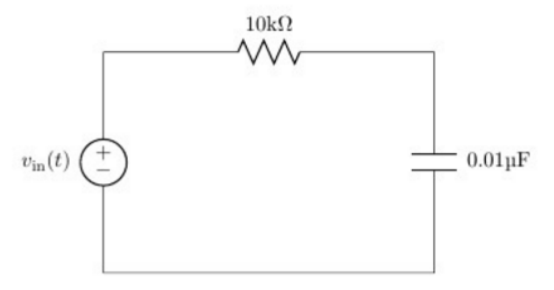
\includegraphics[width=\linewidth]{images/1_1.PNG}
	\caption{RC circuit for square wave input analysis}
	\label{fig:cir}
\end{figure}

We used channel 1 of the oscilloscope to verify the input and measured the output voltage of the capacitor by channel 2. Figure[\ref{fig:osc1}] is the screen output of two and half cycles.

\begin{figure}[!htbp]
	\centering
	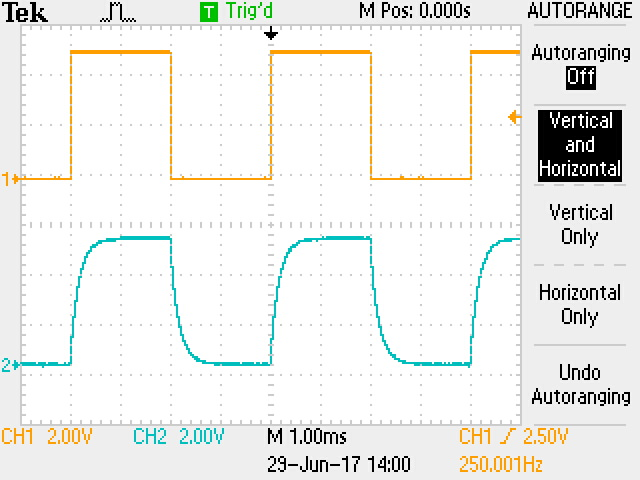
\includegraphics[width=0.95\linewidth]{images/1_2.JPG}
	\caption{The waveform of input and measure}
	\label{fig:osc1}
\end{figure}

\textbf{Analyze \#1:} \newline
\phantom{ } The oscilloscope did display the same waveform plotted in Prelab\#7. They are of the same shape, and both of their peaks and valleys reach the input waveform. Meanwhile, no obvious difference is found. \newline

Using the \textit{Cursor} menu, we recorded the period $T$, as well as the range of the output signal. Then we measured the time value of the $10\%$, $90\%$, and $50\%$ point of $V_{out}$. The results are shown in table[\ref{tab:mea}].

\begin{table}[!htbp]
	\centering
	\caption{Measurements of the output signal}
	\begin{tabular}{lcl}
		\toprule
		name & value & \\
		\midrule
		period & $4.000\mathrm{ms}$ & \\
		max voltage & $5.120\mathrm{V}$ & \\
		min voltage & $0.000\mathrm{V}$ & \\
		time of $10\% V_{out}$ (LH) & $16.0\mathrm{\mu s}$ & \\
		time of $90\% V_{out}$ (LH) & $364\mathrm{\mu s}$ & \\
		time of $50\% V_{out}$ (LH) & $116\mathrm{\mu s}$ & \\
		time of $10\% V_{out}$ (HL) & $??\mathrm{\mu s}$ & \\
		time of $90\% V_{out}$ (HL) & $??\mathrm{\mu s}$ & \\
		time of $50\% V_{out}$ (HL) & $??\mathrm{\mu s}$ & \\
		\bottomrule
	\end{tabular}
	\label{tab:mea}
\end{table}

\textbf{Analysis \#2:} \newline
\phantom{ } After calculating the rise time, fall time, and delay time of the RC circuit, we got table[\ref{tab:cal}].

\begin{table}[!htbp]
	\centering
	\caption{Measurements of the output signal}
	\begin{tabular}{lcccl}
		\toprule
		name & actual value & theoretical value & PE & \\
		\midrule
		rise time & $348\mathrm{\mu s}$ & ${220\mu s}$ & $58.2\%$ & \\
		fall time & $??\mathrm{\mu s}$ &  ${220\mu s}$ & $??\%$ & \\
		delay time (LH) & $116\mathrm{\mu s}$ & ${69\mu s}$ & $68.1\%$ & \\
		delay time (HL) & $??\mathrm{\mu s}$ &  ${69\mu s}$ & $??\%$ & \\
		\bottomrule
	\end{tabular}
	\label{tab:cal}
\end{table}

\textbf{A}
	\subsubsection{Time Constant Measurement}
	\hfill \newline
\phantom{ } After we connected the circuit in Graph[\ref{fig:cir}] in the lab instruction, we detected a waveform on our oscilloscope. To calculate its time constant accurately, we need as many data as possible. According to the instruction, we recorded 10 points separately for the original circuit, two-stage and three-stage. When we were selecting our testing points, we tried to pick more where the voltage rose(or fell) more rapidly with time. Also, we noticed that the measurements were not stable on the oscilloscope if its value was too small, so we paused the screen on random to record a relatively accurate number.\\
\phantom{ } When we were measuring the voltages and their according time, we used the Cursor whose type was time and took Channel 2 as its source. We settle one of the cursor at start point of a rising or falling action, and moved the other cursor slightly. We also scaled the width of the waveform to get a more accurate move.\\
\phantom{ } Our recordings for the original circuit are shown in the table below.

\begin{table}[!htbp]\centering
	\caption{Experiment record in the original circuit}
	\renewcommand\arraystretch{1.5}
	\begin{tabular}{lcl}
		\toprule
		No		&Voltage(V)	&time($\mathrm{\mu s}$)	\\
		\midrule
		1		&0.64		&24.0		\\
		
		2		&1.32		&56.0		\\
		
		3		&1.96		&88.0		\\
		
		4		&2.16		&100		\\
		
		5		&2.76		&140		\\
		
		6		&3.14		&176		\\
		
		7		&3.76		&248		\\
		
		8		&4.20		&340		\\
		
		9		&4.40		&412		\\
		
		10		&4.60		&512		\\
		\bottomrule
	\end{tabular}
\end{table}
\hfill \newline
\textbf{Analyze \#4:} \newline
\phantom{ } Then we applied the data in Excel, we got a plot[\ref{fig:2.1}].\\
\begin{figure}[!htbp]
	\centering %居中
	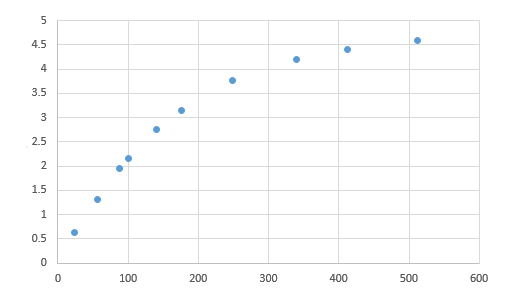
\includegraphics[width=\linewidth]{images/2_1.PNG} %宽度,文件地址
	\caption{Plot on the Voltage of capacitor in the original circuit with time.} %标题
	\label{fig:2.1} %标记(引用时用)
\end{figure}
After we tried to conduct(for details, please check the Appendix) the formula under the Analysis \#4 in the instruction file, we found that we need to adjust the value of y-axis from $V_{out}(t)$ to $\frac{V_0 - V_{out}(t)}{V_0}$ so that the unit of voltage is unrelated to the final result, also leaving the exponential part alone on the right side of the equality mark. Also, it is the y-axis(ratio) that needs to be logarithmic, not x-axis(time). After making y-axis logarithmic, it is equivalent to applying the ln operation to both side of the equation and taking the left side as y. Thus making the right side become $-\frac{t}{\tau}$. Then we can fit the current plot to a linear line and calculate the time constant from the inverse of the line's slope as shown in the graph[\ref{fig:2.2}].\\
\phantom{ }After we tried to conduct the formula under the Analysis \#4 in the instruction file, we found that we need to adjust the value of y-axis from $V_{out}(t)$ to $\frac{V_0 - V_{out}(t)}{V_0}$ so that the unit of voltage is unrelated to the final result, also leaving the exponential part alone on the right side of the equality mark. Also, it is the y-axis(ratio) that needs to be logarithmic, not x-axis(time). After making y-axis logarithmic, it is equivalent to applying the ln operation to both side of the equation and taking the left side as y. Thus making the right side become $-\frac{t}{\tau}$. Then we can fit the current plot to a linear line and calculate the time constant from the inverse of the line's slope as shown in the graph[\ref{fig:2.2}].\\
\begin{figure}[!htbp]
	\centering %居中
	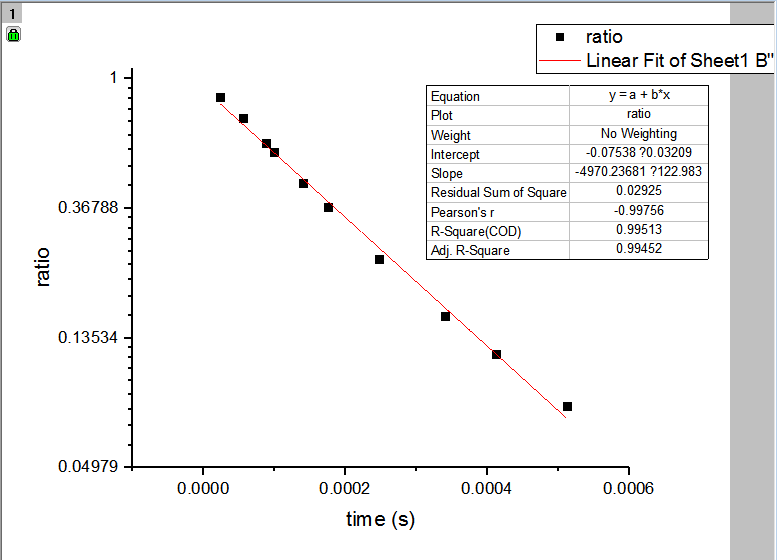
\includegraphics[width=\linewidth]{images/2_2.PNG} %宽度,文件地址
	\caption{plot on the logarithmic ratio ({\tiny }) in the original circuit with time.} %标题
	\label{fig:2.2} %标记(引用时用)
\end{figure}
%\phantom{ } 
Then we fit a linear line to this plot, and we get a slope of -4970.
we got its inverse $2.012\times10^{-4}\mathrm{s}$. Also, we calculated the theoretic value for $\tau$ and got 
$\tau = RC = 10\mathrm{k\Omega} \times 0.01\mathrm{\mu F} = 1\times10^{-4}\mathrm{s}$, which led to a 101\% error.\\
\phantom{ } We think it was pretty strange, so we used the multimeter to measure the actual value of the resistor and capacitor we used in our circuit. From measurement, we found that the real value of resistor was 10.1$\mathrm{k\Omega}$, which was quite near to its printed value 10$\mathrm{k\Omega}$. However, the capacitor's real value had a great error with its printed value. The capacitor we used had an actual capacity of 18.3nF. After we put the real value of our elements into the calculation of theoretical value of time constant, we got
$\tau = RC = 10.1\mathrm{k\Omega} \times 18.3 \mathrm{nF} = 1.85\times10^{-4}\mathrm{s}$, which led to a percent error of 8.76\%, a quite better result than before.\\
\phantom{ } But there are still some difference. We discussed and think that the possible resource of difference might be among the list below:\\
1. The oscilloscope had a measure error on the output signal.(May caused by the interference of the current in the circuit and other reasons)\\
2. The resistor in the cables and experimental boards were not taken into account.\\
3. The capacitor showed an unstable value for its capacity when we measured it, so its capacity may be easily influenced by some factors in the environment(such as temperature).\\
4. The capacitor may act like a resistor or an inductor at extreme frequencies.\\
\newline
\textbf{Analyze \#5:} \newline
\phantom{ } To finish this analysis, we built a two-stage circuit and then a three-stage circuit. Our two-stage circuit is built according to graph[\ref{fig:2.3}].\\
\begin{figure}[!htbp]
	\centering %居中
	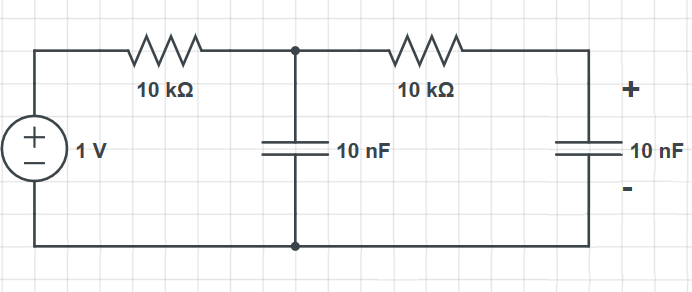
\includegraphics[width=\linewidth]{images/2_3.PNG} %宽度,文件地址
	\caption{The circuit graph of two-stage circuit} %标题
	\label{fig:2.3} %标记(引用时用)
\end{figure}
\phantom{ } In the same way as in the original circuit, we measure 10 points to compute its time constant.
\begin{table}[!htbp]\centering
	\caption{Experiment record in the two-stage circuit}
	\renewcommand\arraystretch{1.5}
	\begin{tabular}{lcr}
		\toprule
		No		&Voltage(V)	&time($\mathrm{\mu s}$)	\\
		\midrule
		1		&0.04		&20.0		\\

		2		&0.08		&30.0		\\
		
		3		&0.16		&50.0		\\
		
		4		&0.48		&90.0		\\
		
		5		&0.80		&130		\\
		
		6		&1.68		&250		\\
		
		7		&2.40		&360		\\
		
		8		&3.04		&500		\\
		
		9		&4.28		&1000		\\
		
		10		&4.72		&1650		\\
		\bottomrule
	\end{tabular}
\end{table}
%\phantom{ } Like in the original circuit, we plot two figures[\ref{fig:2.5},\ref{fig:2.6}] to show the relative of our measures in two-stage.
%\begin{figure}[!htbp]
%	\centering %居中
%	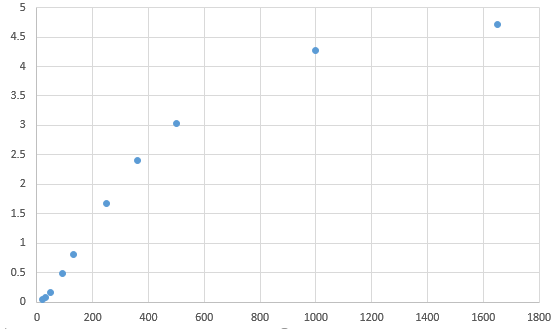
\includegraphics[width=\linewidth]{images/2_5.PNG} %宽度,文件地址
%	\caption{Plot on the Voltage of capacitor in the two-stage circuit with time.} %标题
%	\label{fig:2.5} %标记(引用时用)
%\end{figure}
%\begin{figure}[!htbp]
%	\centering %居中
%	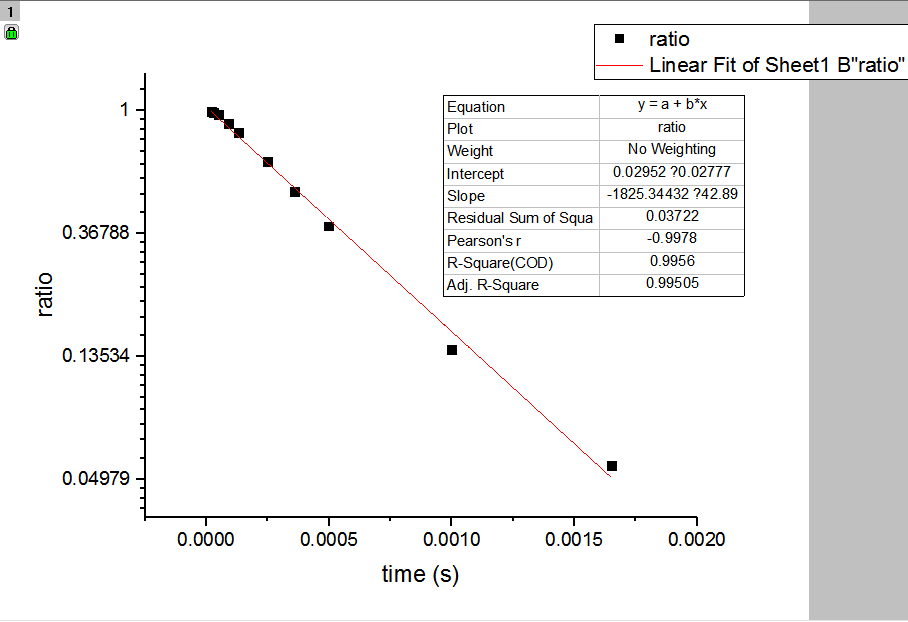
\includegraphics[width=\linewidth]{images/2_6.PNG} %宽度,文件地址
%	\caption{Plot on the logarithmic ratio ({\tiny }) in the two-stage circuit with time.} %标题
%	\label{fig:2.6} %标记(引用时用)
%\end{figure}
\phantom{ } We then get the time constant of two-stage 
$\tau = -\frac{1}{slope} = -\frac{1}{-1825} = 5.479\times10^{-4}$s.\\ And according to the circuit graph and some prelab exercise and the result of our measurement in analysis 4, we can easily compute
the theoretical value of time constant in this case:\\
$\tau = 3RC = 3\times1.85\times10^{-4} = 5.55\times10^{-4}$s and the percent error $error = 1.28\%$.\\
\phantom{ } Our three-stage circuit was built based on graph[\ref{fig:2.4}].\\
\begin{figure}[!htbp]
	\centering %居中
	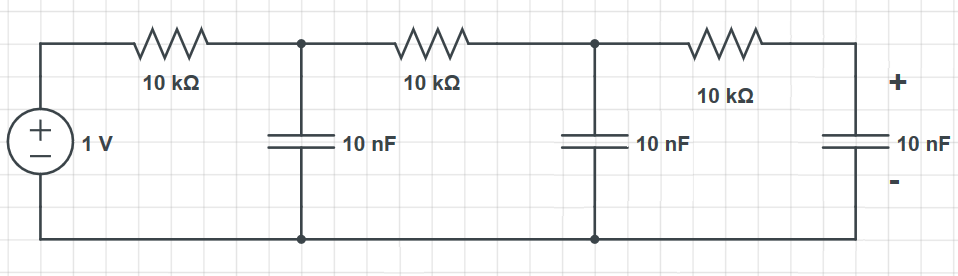
\includegraphics[width=\linewidth]{images/2_4.PNG} %宽度,文件地址
	\caption{The circuit graph of three-stage circuit} %标题
	\label{fig:2.4} %标记(引用时用)
\end{figure}
\phantom{ }And our measure points are listed below:\\
\begin{table}[!htbp]\centering
	\caption{Experiment record in the three-stage circuit}
	\renewcommand\arraystretch{1.5}
	\begin{tabular}{lcr}
		\toprule
		No		&Voltage(V)	&time(ms)	\\
		\midrule
		1		&0.04		&100		\\
		
		2		&0.24		&180		\\
		
		3		&0.52		&250		\\
		
		4		&0.82		&330		\\
		
		5		&1.28		&450		\\
		
		6		&1.80		&600		\\
		
		7		&2.40		&810		\\
		
		8		&3.00		&1110		\\
		
		9		&3.60		&1550		\\
		
		10		&3.92		&1930		\\
		\bottomrule
	\end{tabular}
\end{table}
%\phantom{ } Like in the original circuit, we plot two figures[\ref{fig:2.7},\ref{fig:2.8}] to show the relative of our measures in three-stage.
%\begin{figure}[!htbp]
%	\centering %居中
%	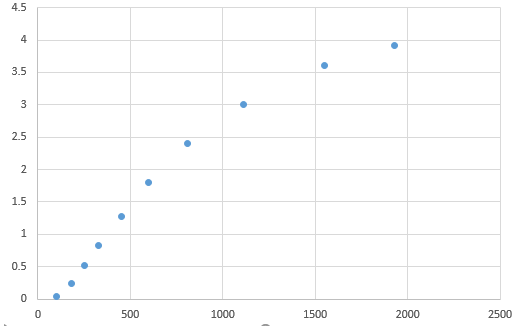
\includegraphics[width=\linewidth]{images/2_7.PNG} %宽度,文件地址
%	\caption{Plot on the Voltage of capacitor in the three-stage circuit with time.} %标题
%	\label{fig:2.7} %标记(引用时用)
%\end{figure}
%\begin{figure}[!htbp]
%	\centering %居中
%	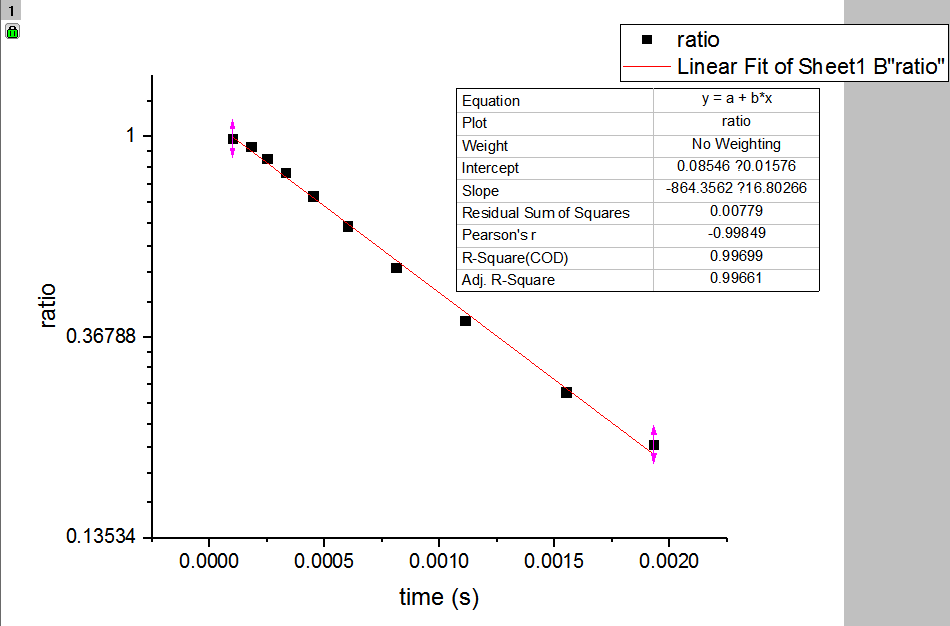
\includegraphics[width=\linewidth]{images/2_8.PNG} %宽度,文件地址
%	\caption{Plot on the logarithmic ratio ({\tiny }) in the three-stage circuit with time.} %标题
%	\label{fig:2.8} %标记(引用时用)
%\end{figure}
\phantom{ } We then get the time constant of three-stage: 
\begin{center}
	$\tau = -\frac{1}{slope} = -\frac{1}{-864.4} = 1.157\times10^{-3}$s
\end{center}

And according to the circuit graph and some prelab exercise, we can easily compute
the theoretical value of time constant in this case:
$\tau = 6RC = 6\times1.85\times10^{-4} = 1.11\times10^{-3}$s and the percent error $error = 4.23\%$.\\
\phantom{ } We thought the reason for the difference may among these reasons:\\
1. Some existing reasons that we have already mentioned in Analysis 4.\\
2. The resistors and capacitors we used to build two-stage and three-stage circuit may be different from those in the original circuit, thus causing some difference.\\
3. Other equipment errors caused by adding more elements and wires in our circuit.\\


	\subsection{The RC Response to a Sinusoidal Input}
	\hfill\newline
%will take care of tex and graphs when the body is finished
%should ask for more experimental details
%revise the sentences!
\phantom{ } The circuit in Figure [] was built again to measure the response to a sinusoidal input. Channel 1 and 2 were connected into the circuit to display the voltage over the input port and the capacitor. Figure [] shows the waveform of these two voltages, as captured from the oscilloscope display. \newline
//figure\\
\phantom{ } To measure the response to signals of various frequencies, we kept the input amplitude at 1V, and swept the input frequency from 10Hz to 1MHz. Table [] shows the recorded amplitudes of the output signals. Figure [] is a plotted figure of the amplitude-frequency data, with a logarithmic scale on the x-axis.\newline
//table\newline
//figure voltage over the capacitor in terms of frequency\\

\textbf{Analyze \#6:} \newline
\phantom{ } Comparing the figure above to what was plotted in prelab\#11, we noticed that the pattern of data we collected in the experiment was consistent with the calculation before. Amplitude decreased rapidly with the frequency increasing in middle range, while the slope was comparatively small with the frequency approaching $10^6$.\\
\phantom{ } However, the curve between $10^4$ and $10^5$ was not very smooth. The error may has occurred when we operated the oscilloscope. We noticed that sometimes moving the cursor on the time axis did not change the value on the screen. The reason might be that the machine measures the graph on it to give out values, which means an unavoidable error from the width of the lines.\\\\
\phantom{ } Next, we changed the output to be the voltage over the resistor, and the function generator to provide a sinusoidal wave with 1V amplitude. Table [] shows the amplitudes recorded under various frequencies, and they are plotted in the figure Fig[].\newline
//table\newline
//fig voltage over the resistor in terms of frequency\\

\textbf{Analyze \#7:} \newline

	\section{Conclusions}
	\phantom{ } We completed all the circuit building and measurements required in this lab, and got a result that fit our computation result in prelab. We also used our result to finish the analysis part in this lab, which gave us some hints to do our lab with more efficiency. \\
\begin{table}[!htbp]
	\caption{Team Roles}
	\renewcommand\arraystretch{1.5}\centering
	\begin{tabular}{l|c}
		\hline
		\hline
		Activity					&	Student Name 	\\
		\hline
		Prelab/Circuit Analysis		& 	Muhan Li		\\
		\hline
		Prelab/Simulations			&	Mingxiao An		\\
		\hline
		Prelab/answer questions		&	Man Sun			\\
		\hline
		Circuit construction		&	Mingxiao An		\\
		\hline
		Data collection				& Muhan Li, Man Sun	\\
		\hline
		Data analysis				& Muhan Li, Man Sun \\
		\hline
		Lab report writing			& Mingxiao An, Muhan Li, Man Sun \\
		\hline
		\hline
	\end{tabular}\\
\end{table}
	\section{Appendix}
	\textbf{Procedure of conduction in Analysis \#4:}  \newline
\phantom{ } From the lab instruction, we get a formula\\
\begin{center}
	$Ratio(t) = \frac{|v_{out}(t) - v_{in}|}{|V_0|} = e^{-\frac{t}{\tau}}$\\
\end{center}
\phantom{ } In the process of rising, we can take $v_{in}$ as $V_0$, because it stays at this value during the whole rising process. Because the whole rising process shows that the capacitor is charging, which means that $v_{out} - V_0 < 0$ holds true during the whole rising while $V_0 > 0$ is always true in this case.Then we conducted our 
computation for Ratio(t).\\

\begin{center}
$Ratio(t) = \frac{V_0 - v_{out}(t)}{V_0} = 1 - \frac{v_{out}(t)}{V_0}$
\end{center}

\phantom{ } Then, if we apply $\ln$ operation to the Ratio(t) and exponential part, we get 
	$\ln(Ratio(t)) = -\frac{t}{\tau}$.
So the exponential part becomes linear, which is easy to analysis.\\
	
\end{document}
